\documentclass{beamer}
\usetheme{Boadilla}
\usecolortheme{dolphin}
\usepackage{amsmath}
\usepackage{cancel}
\setbeamercovered{invisible}

\newtheorem*{remark}{Remark}

\begin{document}

\begin{frame}
  \frametitle{What Are Prime Numbers?}
  \begin{definition}
    A \alert{prime number} is a number that has exactly two divisors.
  \end{definition}
\end{frame}

\begin{frame}{replacing content}
  \begin{overprint}
    \onslide<1>
    \begin{align*}
      S = A + B
    \end{align*}
    \onslide<2>
    \begin{align*}
      S = A + B'
    \end{align*}
  \end{overprint}

\begin{itemize}[<+->]
\item A
\item B
\end{itemize}

\begin{itemize}[<+-|alert@+>]
\item A
\item B
\end{itemize}

\end{frame}


\begin{frame}<1-3>[label=framelabel]{Taking Detours}
  \begin{itemize}
  \item A
    \pause
  \item B
    \pause
  \item\alert<4->{Something important.
  }
  \end{itemize}
\end{frame}

\

\begin{frame}
  Transition text
  \begin{itemize}
  \item \only<1>{Problem: Here is a problem.}\visible<2>{Solution: Here is a solution.}
  \end{itemize}
  \begin{equation*} y = 2x + \onslide<2->{3} \end{equation*}
  \begin{align*} y = 2x + \onslide<2->{3} \end{align*}
  
\end{frame}

\againframe<4>{framelabel}

\begin{frame}
    \begin{block}{Block Title}
    Lorem ipsum dolor sit amet, consectetur adipisicing elit, sed do eiusmod tempor incididunt ut labore et dolore magna aliqua.
  \end{block}
  \begin{alertblock}{Block Title}
    Lorem ipsum dolor sit amet, consectetur adipisicing elit, sed do eiusmod tempor incididunt ut labore et dolore magna aliqua.
  \end{alertblock}
  \begin{example}
    Lorem ipsum dolor sit amet, consectetur adipisicing elit, sed do eiusmod tempor incididunt ut labore et dolore magna aliqua.
  \end{example}
\end{frame}


\begin{frame}
  \begin{theorem}[about beamer]
    Beamer rocks!
  \end{theorem}
  \begin{remark}[Some important remark]
    Some text
  \end{remark}
\end{frame}

\begin{frame}
    \begin{columns}
      \column{0.38\linewidth}
      \centering
      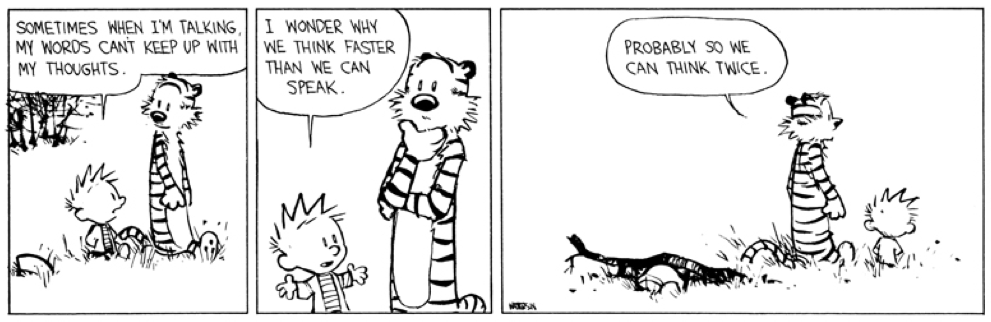
\includegraphics[height=5cm, width=3.5cm]{calvin.png}
      \column{0.58\linewidth}
      \textbf{William George Horner} (geboren in 1786, gestorven in 1837) was een Brits
      wiskundige. Hij studeerde aan de Kingswood School in Bristol, waar hij reeds op
      14(!)-jarige leeftijd een masteropleiding volgde. Daarna trok hij richting Bath
      waar hij een school stichtte.
    \end{columns}
\end{frame}

\end{document}
